\section{Ejercicio 4}
  		Computaciones para el programa
  		\begin{verbatim}
		J(1,4,10)
		T(1,4)
		S(2)
		J(1,2,10)
		Z(3)
		S(3)
		S(4)
		J(1,3,3)
		J(1,1,6)
		T(4,1)
  		\end{verbatim}
  		\subsection{Computación para la entrada $R1=0$}
  		\begin{equation*}\begin{gathered}
		(1, <R1=0, R2=0, R3=0, R4=0>) \sim (10, <R1=0, R2=0, R3=0, R4=0>) \sim\\
		(11, <R1=0, R2=0, R3=0, R4=0>)
		\end{gathered}\end{equation*}
		\begin{figure}[H]
  			\centering
  			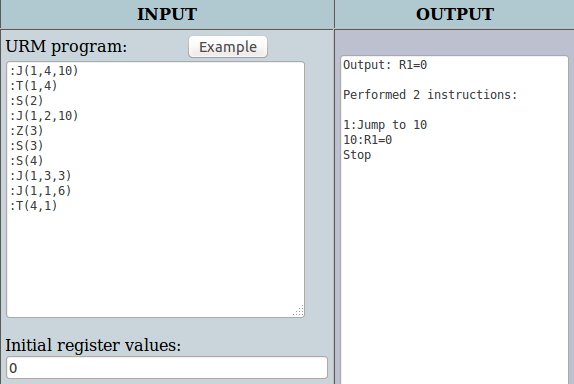
\includegraphics[scale=0.5]{images/40.png}
  		\end{figure}
		\subsection{Computación para la entrada $R1=1$}
  		\begin{equation*}\begin{gathered}
		(1, <R1=1, R2=0, R3=0, R4=0>) \sim (2, <R1=1, R2=0, R3=0, R4=0>) \sim\\
		(3, <R1=1, R2=0, R3=0, R4=1>) \sim (4, <R1=1, R2=1, R3=0, R4=1>) \sim\\
		(10, <R1=1, R2=1, R3=0, R4=1>) \sim (11, <R1=1, R2=1, R3=0, R4=1>)
		\end{gathered}\end{equation*}
		\begin{figure}[H]
  			\centering
  			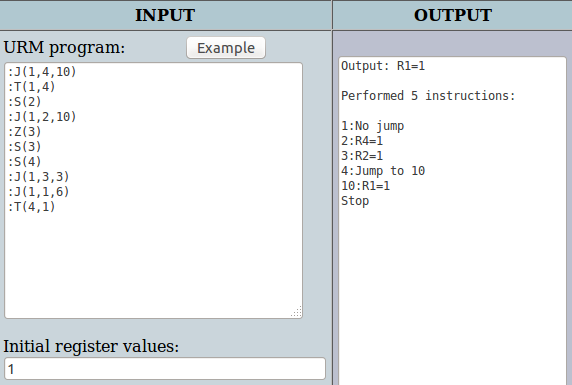
\includegraphics[scale=0.5]{images/41.png}
  		\end{figure}
		\subsection{Computación para la entrada $R1=2$}
		\begin{equation*}\begin{gathered}
		(1, <R1=2, R2=0, R3=0, R4=0>) \sim (2, <R1=2, R2=0, R3=0, R4=0>) \sim\\
		(3, <R1=2, R2=0, R3=0, R4=2>) \sim (4, <R1=2, R2=1, R3=0, R4=2>) \sim\\
		(5, <R1=2, R2=1, R3=0, R4=2>) \sim (6, <R1=2, R2=1, R3=0, R4=2>) \sim\\
		(7, <R1=2, R2=1, R3=1, R4=2>) \sim (8, <R1=2, R2=1, R3=1, R4=3>) \sim\\ 
		(9, <R1=2, R2=1, R3=1, R4=3>) \sim (6, <R1=2, R2=1, R3=1, R4=3>) \sim\\
		(7, <R1=2, R2=1, R3=2, R4=3>) \sim (8, <R1=2, R2=1, R3=2, R4=4>) \sim\\
		(3, <R1=2, R2=1, R3=2, R4=4>) \sim (4, <R1=2, R2=2, R3=2, R4=4>) \sim\\
		(10, <R1=2, R2=2, R3=2, R4=4>) \sim (11, <R1=4, R2=2, R3=2, R4=4>)
		\end{gathered}\end{equation*}
		\begin{figure}[H]
  			\centering
  			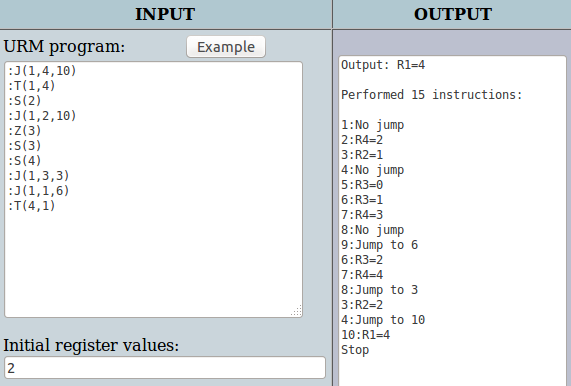
\includegraphics[scale=0.5]{images/42.png}
  		\end{figure}
		\subsection{Computación para la entrada $R1=3$}
		\begin{equation*}\begin{gathered}
		(1, <R1=3, R2=0, R3=0, R4=0>) \sim (2, <R1=3, R2=0, R3=0, R4=0>) \sim\\
		(3, <R1=3, R2=0, R3=0, R4=3>) \sim (4, <R1=3, R2=1, R3=0, R4=3>) \sim\\
		(5, <R1=3, R2=1, R3=0, R4=3>) \sim (6, <R1=3, R2=1, R3=0, R4=3>) \sim\\
		(7, <R1=3, R2=1, R3=1, R4=3>) \sim (8, <R1=3, R2=1, R3=1, R4=4>) \sim\\
		(9, <R1=3, R2=1, R3=1, R4=4>) \sim (6, <R1=3, R2=1, R3=1, R4=4>) \sim\\
		(7, <R1=3, R2=1, R3=2, R4=4>) \sim (8, <R1=3, R2=1, R3=2, R4=5>) \sim\\
		(9, <R1=3, R2=1, R3=2, R4=5>) \sim (6, <R1=3, R2=1, R3=2, R4=5>) \sim\\
		(7, <R1=3, R2=1, R3=3, R4=5>) \sim (8, <R1=3, R2=1, R3=3, R4=6>) \sim\\
		(3, <R1=3, R2=1, R3=3, R4=6>) \sim (4, <R1=3, R2=2, R3=3, R4=6>) \sim\\
		(5, <R1=3, R2=2, R3=3, R4=6>) \sim (6, <R1=3, R2=2, R3=0, R4=6>) \sim\\
		(7, <R1=3, R2=2, R3=1, R4=6>) \sim (8, <R1=3, R2=2, R3=1, R4=7>) \sim\\
		(9, <R1=3, R2=2, R3=1, R4=7>) \sim (6, <R1=3, R2=2, R3=1, R4=7>) \sim\\
		(7, <R1=3, R2=2, R3=2, R4=7>) \sim (8, <R1=3, R2=2, R3=2, R4=8>) \sim\\
		(9, <R1=3, R2=2, R3=2, R4=8>) \sim (6, <R1=3, R2=2, R3=2, R4=8>) \sim\\
		(7, <R1=3, R2=2, R3=3, R4=8>) \sim (8, <R1=3, R2=2, R3=3, R4=9>) \sim\\
		(3, <R1=3, R2=2, R3=3, R4=9>) \sim (4, <R1=3, R2=3, R3=3, R4=9>) \sim\\
		(10, <R1=3, R2=3, R3=3, R4=9>) \sim (11, <R1=9, R2=3, R3=3, R4=9>)
		\end{gathered}\end{equation*}
		\begin{figure}[H]
  			\centering
  			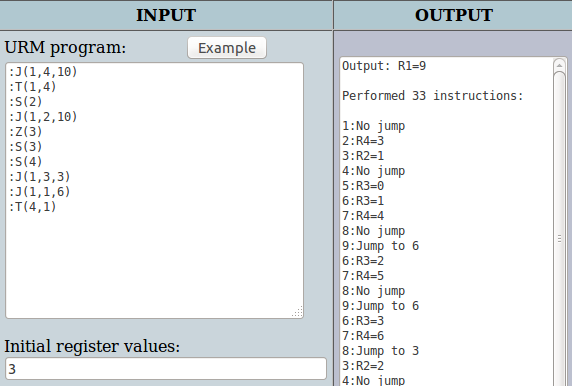
\includegraphics[scale=0.5]{images/43.png}
  		\end{figure}
		\subsection{Función calculada}
		El programa calcula la función
		\begin{equation*}
  			f(x) = x*x
  		\end{equation*}
